\documentclass[tikz,border=10pt]{standalone}
\usepackage{mathrsfs}
\usepackage{physics}
\usetikzlibrary{decorations.pathmorphing}
    % this is for graphics. e.g. rectangle on title page
\usetikzlibrary{3d}
\usetikzlibrary{backgrounds}
\usetikzlibrary{arrows,shapes,positioning,shadows,trees,mindmap}
\usetikzlibrary{tikzmark}
\usetikzlibrary{calc,math}

\usepackage{tikz-3dplot}
\usepackage{pgfplots}
\pgfplotsset{compat = newest}
%\usepgfplotslibrary{colormaps}
\usepgflibrary{shapes.geometric}

\usepackage[edges]{forest}
\usetikzlibrary{arrows.meta}
\colorlet{linecol}{black!75}
\usepackage{xkcdcolors} % xkcd colors

\usetikzlibrary{patterns}
\tikzset{>={Stealth[inset=0pt,angle=20:10pt]}}


\tikzset{zigzag/.style={decorate,decoration=zigzag}}


\begin{document}
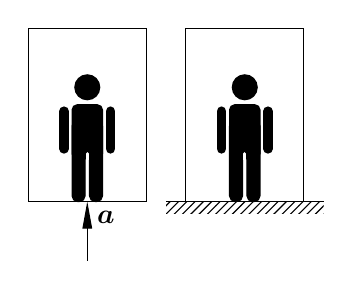
\begin{tikzpicture}



    \draw (-0.75cm,-1.45cm)--(0.75cm,-1.45cm)--(0.75cm,0.75cm)--(-0.75cm,0.75cm)--cycle;
        \node[circle,fill,minimum size=2.5mm] (head) {};
\node[rounded corners=2pt,minimum height=0.7cm,minimum width=0.4cm,fill,below = 1pt of head] (body) {};
\draw[line width=1.25mm,round cap-round cap] ([shift={(-2.5pt,-1pt)}]body.north west)--++(-90:6mm);
\draw[line width=1.25mm,round cap-round cap] ([shift={(2.5pt,-1pt)}]body.north east) --++(-90:6mm);
\draw[rounded corners=2pt,fill] ([shift={(-0.8pt,0.5cm)}]body.south) rectangle (-0.1933cm,-1.45cm);
\draw[rounded corners=2pt,fill] ([shift={(0.8pt,0.5cm)}]body.south) rectangle (0.1933cm,-1.45cm);
\draw[very thick,white,-round cap] (body.south) --++(90:1mm);
\draw[->] (0,-2.2cm)--(0,-1.45cm) node[below right]{$\vb*{a}$};

\begin{scope}[xshift=2cm]
    \draw (-1cm,-1.45cm)--(1cm,-1.45cm);
    \fill[pattern=north east lines] (-1cm,-1.45cm) -- (1cm,-1.45cm) -- (1cm,-1.6cm) -- (-1cm,-1.6cm);
    \draw (-0.75cm,-1.45cm)--(0.75cm,-1.45cm)--(0.75cm,0.75cm)--(-0.75cm,0.75cm)--cycle;
        \node[circle,fill,minimum size=2.5mm] (head) {};
\node[rounded corners=2pt,minimum height=0.7cm,minimum width=0.4cm,fill,below = 1pt of head] (body) {};
\draw[line width=1.25mm,round cap-round cap] ([shift={(-2.5pt,-1pt)}]body.north west)--++(-90:6mm);
\draw[line width=1.25mm,round cap-round cap] ([shift={(2.5pt,-1pt)}]body.north east) --++(-90:6mm);
\draw[rounded corners=2pt,fill] ([shift={(-0.8pt,0.5cm)}]body.south) rectangle (-0.1933cm,-1.45cm);
\draw[rounded corners=2pt,fill] ([shift={(0.8pt,0.5cm)}]body.south) rectangle (0.1933cm,-1.45cm);
\draw[very thick,white,-round cap] (body.south) --++(90:1mm);
\end{scope}
    \end{tikzpicture}
\end{document}